\documentclass{beamer}
\usepackage{times}
\usepackage{fontspec}
\usepackage{ctex, hyperref}
\usepackage{subfig}
\usepackage{amssymb,amsmath,mathtools}
\usepackage{amsfonts,booktabs}
\usepackage{lmodern,textcomp}
\usepackage{color}
\usepackage{multicol}
\usepackage[utf8]{inputenc}
\usepackage{natbib}
\usepackage{multirow}
\usepackage{float}
\usepackage{bbding}
\usepackage{array}
\usepackage{tikz}
\usepackage{url}% 超链接
\let\Tiny\tiny
\beamertemplatenavigationsymbolsempty
\usetheme{Madrid}
% \usetheme{Warsaw}
% \usetheme{Darmstadt}
% \usetheme{Rochester}
% \usetheme{Frankfurt}
% \usetheme{CambridgeUS}
% \usetheme{default}
% \usefonttheme{serif} %times new roman
\definecolor{Green}{RGB}{43,134,75}
\usecolortheme{naugreen}
\setbeamercolor{item projected}{bg=Green,fg=white}
% \definecolor{UBCblue}{rgb}{0.04706, 0.13725, 0.26667} % UBC Blue (primary)
\usefonttheme[onlymath]{serif}

\newfontfamily\chalkd{Times New Roman}

\setbeamerfont{normal text}{family=\chalkd,series=\mdseries}
\setbeamerfont{alerted text}{family=\chalkd,series=\bfseries}
\setbeamerfont{frametitle}{family=\chalkd,series=\bfseries}


\begin{document}
\usebeamerfont{normal text}
\title[Place]{ {联邦学习的开山之作}}
\author[Z.Y. Li]{\songti 李志远}
\institute[NAU]{
    % \large
    {
\includegraphics[scale=0.3]{images/naulogo.png}} \\
    \songti{南京农业大学\,\,\,人工智能学院\,\,\,人工智能201}
}
\date[\songti \fontsize{7pt}{5pt}{\today}]{\fangsong \fontsize{10pt}{5pt}{\today}}


\addtobeamertemplate{frametitle}{}{%
\begin{tikzpicture}[remember picture,overlay]
\node[anchor=north east,yshift=2pt, xshift=7pt] at (current page.north east) {
\includegraphics[scale=0.3]{images/logo.png}};
\end{tikzpicture}
\vspace{-10pt}
}

\AtBeginSection[]
{
  \begin{frame}
    \frametitle{\songti \color{white}目录}
    \tableofcontents[currentsection]
  \end{frame}
}
\frame{\titlepage}

\songti

\section{导言}
\subsection{问题来源}
\begin{frame}{\songti 问题来源}
    \begin{tikzpicture}[remember picture,overlay]
        \node[anchor=north,yshift=-25pt, xshift=0pt] at (current page.north) {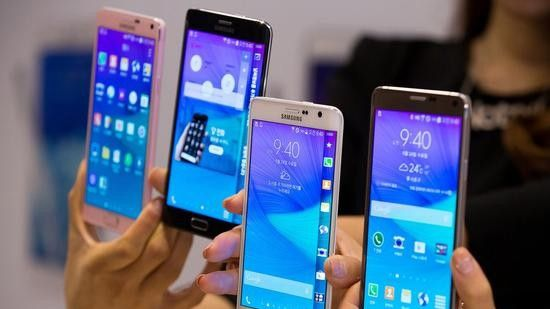
\includegraphics[scale=0.35]{images/phone.png}};
    \end{tikzpicture}
    \vspace{2.5cm}
    \begin{itemize}
        \item 移动设备拥有巨量的可供模型学习的数据,学习这些数据能够为使用设备的人极大地{\color{red}{ \textbf{提升用户体验}}}
        \item 问题:这些数据是{\color{red} \textbf{敏感的、私密的}},而且数量很大;这会对录入服务器后使用传统的方法训练有一定的影响。
    \end{itemize}
\end{frame}

\subsection{其他解决方案(related works)}
\begin{frame}{\songti 其他解决方案}
    \begin{itemize}
        \item 没有考虑\textbf{不平衡}和\textbf{非iid数据}
            \begin{itemize}
                \item McDonald和Povey分别针对感知机和语音识别dnn通过迭代平均本地的训练模型进行分布式训练
                \item Zhang研究了一种soft平均的异步方法
                \item Shokri和Shmatikov的工作在几个方面是相关的:他们专注于训练深度网络,强调隐私的重要性,并通过在每一轮通信中仅共享参数的子集来解决通信成本
            \end{itemize}
        \item Neverova等人也讨论了\textbf{使敏感用户数据留在设备上}的优点。
        \item 分布式共识算法放松了IID假设,但仍然不适合在非常多的客户端上进行通信约束优化。
        \item 已经证实的:\textbf{每个客户端都求解最小化(可能是正则化的)局部数据损失的模型,这些模型被平均以产生最终的全局模型}。这种方法已经在IID数据的凸案例中得到了广泛的研究,并且已知在最坏情况下,生成的全局模型并不比在单个客户端上训练模型好。
    \end{itemize}
\end{frame}

\subsection{联邦学习}
\begin{frame}{\songti 联邦学习定义}
    \begin{tikzpicture}[remember picture,overlay]
        \node[anchor=north,yshift=-25pt, xshift=0pt] at (current page.north) {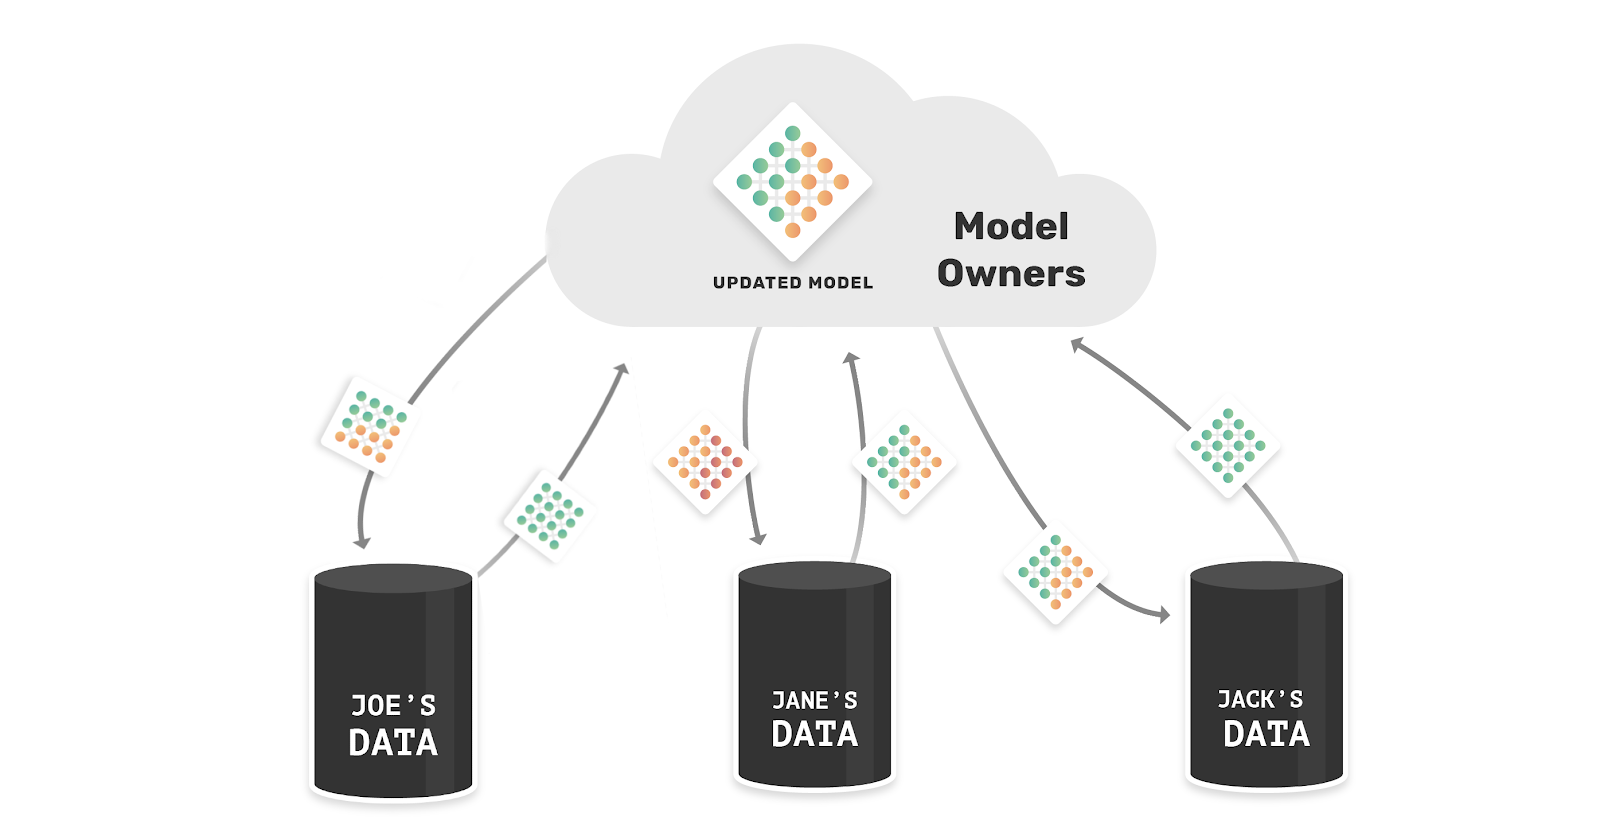
\includegraphics[scale=0.11]{images/federate learning.png}};
    \end{tikzpicture}
    \vspace{65pt}
    \begin{itemize}
        \item {\fontsize{8pt}{2pt}将训练数据分布在移动设备上(即不移动用户数据),通过在移动设备上进行训练、更新参数,将模型的参数传回服务器,来学习一个共享模型。我们将这种分散分布的方法称为\textbf{联邦学习}}
        \vspace{-3pt}
        \item {\fontsize{8pt}{2pt}联邦学习名字由来:问题是通过参与设备(client)的松散联合(federation)解决的,由中央服务器(server)协调。每个client有局部的训练数据集,该数据集绝不上传到server。server维护一个全局的模型,client计算模型的更新,\textbf{仅通信这个更新}。}
        \vspace{-3pt}
        \item {\fontsize{8pt}{2pt}联邦学习的优点:\textbf{将模型训练与直接访问训练数据解耦},两者不再必需;训练数据不必上传到服务器除了用户本身隐私会得到很大程度的保护之外,更重要的是,如果数据本身带有攻击性,那么它带来的伤害就会最大程度的减少,联邦学习可以将攻击面仅限制在当前设备上,而不是设备和云上。}
    \end{itemize}
\end{frame}
\begin{frame}{\songti 隐私}
    \begin{itemize}
        \item 与数据中心对持久数据进行训练相比,联邦学习具有明显的隐私优势。即使持有一个“匿名”数据集,通过与其他数据的关联仍然会将用户的隐私置于风险之中
        \item 为联邦学习传输的信息是改进特定模型所需的\textbf{最小更新}(隐私保护的强度取决于更新的内容)。
        \begin{itemize}
            \item 例如,如果更新是所有本地数据损失的总梯度,并且特征是一个\textbf{稀疏}的词袋,那么非零梯度准确地揭示了用户在设备上输入了哪些单词。相比之下,\textbf{密集模型}(如CNN)的许多梯度的总和为寻求单个训练实例信息的攻击者提供了一个更难的目标(尽管攻击仍然是可能的)。
        \end{itemize}
    \end{itemize}
\end{frame}
\begin{frame}{\songti 联邦学习应用场景}
    \begin{itemize}
        \item 应用场景
        \begin{itemize}
            \item \textbf{在来自移动设备的真实数据上进行训练比在数据中心通常可用的代理数据上进行训练具有明显的优势}。
            \item 这些数据对隐私敏感,或者大小很大(与模型的大小相比),因此最好不要纯粹为了模型训练的目的将其记录到数据中心(为集中收集原则服务)。
            \item 对于监督任务,数据上的标签可以从用户交互中自然地推断出来。
        \end{itemize}
        \item 支持上述场景的模型例子
        \begin{itemize}
            \item 图片分类模型:预测哪种图片流行
            \item 语言模型:语音识别、文本输入(通过训练解码、下一个词的预测、QA来提高精度)
            \item 这两项任务的训练数据可能是隐私敏感的(密码、url、消息等),而且数据的分布也与其他代替数据集有很大的不同。这些问题的标签是直接可用的:输入的文本是自标记的,用于学习语言模型,照片标签可以通过用户与他们的照片app的交互来定义(照片被删除、共享或查看)。两个任务均有出色的模型可用,图片分类模型使用cnn,语言模型使用rnn(2017年transformer还没火)
        \end{itemize}
    \end{itemize}
\end{frame}


\section{联邦平均算法}
\subsection{联邦优化}
\begin{frame}{\songti 联邦优化基本内容}
    \begin{itemize}
        \item 定义:我们将联邦学习中隐含的优化问题称为\textbf{联邦优化},并将其与分布式优化联系起来(并进行对比)。
        \item 区别于典型的分布式优化问题的关键属性
        \begin{itemize}
            \item \textbf{Non-IID} 在给定client上的训练数据通常基于特定用户的移动设备的使用情况,因此任何使用者的本地数据集都不能代表总体分布
            \item \textbf{Unbalanced} 一些用户的数据集会比其他用户大很多(他们使用设备更频繁)
            \item \textbf{Massively distributed}(大规模分布)参与优化的客户端数量远大于每个客户端的平均实例数量
            \item \textbf{Limited communication} 移动设备会频繁掉线、速度缓慢、费用昂贵
        \end{itemize}
        \item 我们任务的重点是在\textbf{非独立同分布和不平衡}的数据上的性能优化,还有\textbf{针对通信约束}的关键优化。一个部署的联邦优化系统还要解决无数的实际问题
    \end{itemize}
\end{frame}
\begin{frame}{\songti 联邦优化特点}
    \begin{itemize}
        \item 联邦优化不同于数据中心优化,其通信成本远大于计算成本,client的训练环境、训练时间都有一定的限制。由于本地数据集远小于整体数据集,因此计算相对于通信的成本来讲基本是免费的,所以本文计划通过增添额外的计算来减少训练模型所需的通信轮次并给出了两个主要的方式:
        \begin{itemize}
            \item 增加并行性,在每个通信轮次内我们使用更多的client执行计算
            \item 每个client上的计算量增加,每个client在每轮通信执行更复杂的计算,而不是执行像梯度计算这样的简单计算。
        \end{itemize}
        \item 本文对两种方法都进行了研究,\textbf{但实现的加速主要是由于在每个client上增加了更多的计算}。
    \end{itemize}
\end{frame}

\subsection{算法简介}
\begin{frame}{\songti 算法简介}
    \begin{tikzpicture}[remember picture,overlay]
        \node[anchor=north,yshift=-25pt, xshift=0pt] at (current page.north) {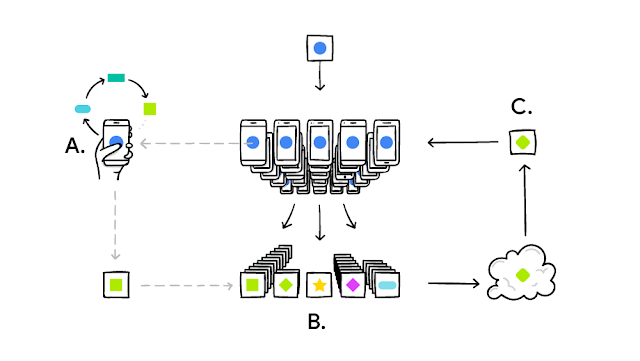
\includegraphics[scale=0.4]{images/image.png}};
    \end{tikzpicture}
    \vspace{80pt}
    \begin{itemize}
        \item 从SGD开始构建
        \item \textbf{FederatedSGD}:global batch size=C,每一轮选择一部分client计算其持有的全部数据的梯度,选择比率为C,C=1时即选择全部数据进行梯度下降(即full-batch gradient descent)
    \end{itemize}
\end{frame}
\begin{frame}{FederatedSGD Baseline {\songti 实现}}
\begin{itemize}
    \item $C=1 \quad learning rate=\eta$,对每个$client\,\, k$计算$g_k=\nabla F_k(w_t)$ 基于当前模型参数$w_t$、本地数据计算的平均梯度。
    
    \begin{minipage}{0.9\textwidth}
    \centering
    \begin{block}{\songti \fontsize{12pt}{9pt}两种更新过程}
        \begin{equation}
            w_{t+1}\leftarrow{{w_{t}}}-{{\eta}}\sum_{k=1}^{K}\frac{n_{k}}{n}{{g_{k}}}
        \end{equation}
        \begin{equation}
            \forall k,w^k_{t+1}\leftarrow w_t-\eta g_k \text{ then } w_{t+1}\leftarrow\sum_{k=1}^K\frac{n_k}{n}w_{t+1}^k
        \end{equation}
    \end{block}
    \end{minipage}  
    \item 一旦算法以这种方式编写,我们就可以\textbf{在梯度平均步骤之前多次迭代本地更新}$$w^k\leftarrow w^k-\eta\nabla F_k(w^k)$$从而为每个client增加更多的计算量。
\end{itemize}
\end{frame}
\begin{frame}{\songti 更新次数的计算}
\begin{itemize}
    \item 上述过程即为FederatedAveraging,计算量由三个关键参数控制:
    \begin{itemize}
        \item \textbf{C},每轮执行计算的client比例
        \item \textbf{E},则每个客户端在每一轮中对其本地数据集进行的训练数
        \item \textbf{B}, 用于客户端更新的本地小批量大小。
    \end{itemize}
    \item 我们将$B =\infty$表示整个本地数据集被视为单个小批量处理。因此,我们可以取$B =\infty$和$E = 1$作为这个算法族的一个端点,这恰好对应于刚刚实现的FedSGD。对于有$n_k$个本地示例的客户端,每轮本地更新的数量为\\
    \centering
    \begin{minipage}{0.6\textwidth}
    \begin{block}{\songti \fontsize{9pt}{9pt} 更新数量}
        \begin{equation}
            u_k = E \frac{n_k}{B}
        \end{equation}
    \end{block}
    \end{minipage}
\end{itemize}
\end{frame}
\begin{frame}{\songti 伪代码}
    \begin{tikzpicture}[remember picture,overlay]
        \node[anchor=north,yshift=-25pt, xshift=0pt] at (current page.north) {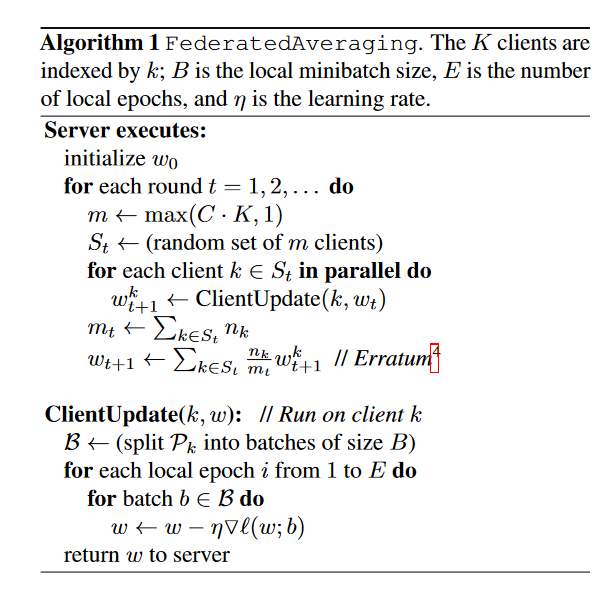
\includegraphics[scale=0.81]{images/federateavg.png}};
    \end{tikzpicture}
\end{frame}

\section{实验}
\begin{frame}{实验总结}
    \begin{itemize}
        \item 我们的动机来自于图像分类和语言建模任务,其中良好的模型可以极大地提高移动设备的可用性。对每一个任务选择大小合适的代理数据集使得能够研究FedAvg算法的超参数。训练了2000多个独立的模型并给出CIFAR-10图像分类任务的结果。最后在一个大型语言建模任务上进行了评估。
        \item MNIST图像分类实验:
        \begin{itemize}
            \item 两个模型 一个多层感知机,一个卷积
            \item 两种数据分布 一种IID(独立同分布),一种非IID
            \begin{itemize}
                \item \textbf{IID设置:数据随机打乱,100个client每个接受600个样本}
                \item \textbf{非IID设置:数据按照标签排序,按顺序分成200个300大小的组,每个client接受2个组,这样每个client最多有2个数字标签,分布很差。}
            \end{itemize}
        \end{itemize}
    \end{itemize}
\end{frame}
\begin{frame}{CIFAR {\songti 结果}}
    \begin{itemize}
        \item 模型取自tensorflow tutorial
    \end{itemize}
    \begin{figure}
        \centering
        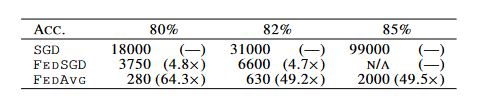
\includegraphics[scale=0.7]{images/CIFARresult.png}
    \end{figure}
\end{frame}
\begin{frame}{LM {\songti 结果}}
    \begin{itemize}
        \item 数据集:社交网络的1000万个公开帖子,以作者为单位分组,有50万左右的client
        \item 精度定义:在来自不同作者(非训练作者)的1e5篇文章的测试集上报告准确率(在10000种可能性中,预测下一个正确单词概率最高的数据的比例)。
        \item 结果:(每轮在200个客户端上进行训练)
        \begin{figure}
            \centering
            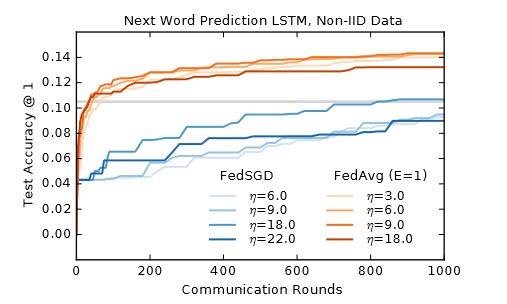
\includegraphics[scale=0.46]{images/LMresult.png}
        \end{figure}
    \end{itemize}
\end{frame}

\section{总结及未来工作}
\begin{frame}{总结及未来工作}
    \begin{itemize}
        \item 我们的实验表明,\textbf{联邦学习可以实现},因为FedAvg使用相对较少的通信轮来训练高质量的模型,在各种模型架构上的结果证明了这一点:一个多层感知器,两个不同的卷积nn,一个两层字符LSTM和一个大规模的词级LSTM。
        \item 通过\textbf{差分隐私}来提供更强的保障、安全多方计算协议、或者他们的结合将是一个有趣的未来工作的方向。注意,这两类技术最自然地应用于像FedAvg这样的同步算法。
        \item 论文的贡献
        \begin{itemize}
            \item 造福后人:发现移动设备分散数据上进行训练是一个重要的研究方向
            \item 选择了一个能够应用于这种设置的简单实用的算法
            \item 对提出的方法进行了广泛的实证评估。
        \end{itemize}
    \end{itemize}
\end{frame}




\begin{frame}
    \fontsize{47.7pt}{1pt}{\centerline{\kaishu 感谢聆听}}
\end{frame}



\bibliography{references}
\bibliographystyle{acl_natbib}
\end{document}